\section{Neural Network}
Neural Network terinspirasi dari cara kerja neuron yang ada pada otak manusia, neuron bertugas sebagai penerima stimulus/rangsangan dan pengirim informasi yang akan diolah atau diproses oleh otak menjadi suatu output. Neuron merupakan sistem saraf pusat dan terdapat sekitar 100 miliar neuron yang ada pada tubuh manusia. Perhatikan gambar \ref{neuron}
\begin{figure}[!htbp]
        \centerline{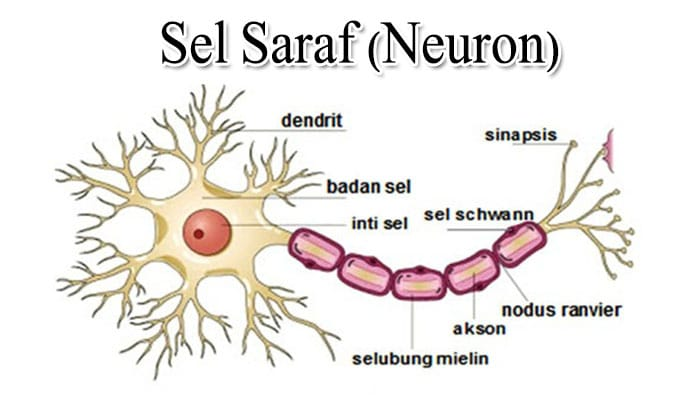
\includegraphics[scale=.45]{figures/neuron}}
        \caption{Sel Saraf (Neuron)}
		\label{neuron}
\end{figure}

Neuron terdiri dari 3 bagian yaitu akson (akar), soma (batang), dan dendrite (cabang). Neuron juga dibedakan menjadi 3 yaitu neuron sensorik atau sel saraf indra karena fungsinya yang berhubungan dengan penerima (indra) dan saraf pusat (otak dan sumsum tulang belakang). Neuron motorik atau sel saraf penggerak yang berfungsi membawa rangsangan dari saraf pusat (otak dan sumsum tulang belakang) ke otot. dan yang terakhir yaitu neuron asosiasi ataus sel saraf penghubung, sel ini menghubungkan atau meneruskan rangsangan dari sel saraf sensorik ke sel saraf motorik.

Tiap neuron yang ada dalam otak kita saling terhubung dan berkirim informasi atau rangsangan berupa neurotransmitter, neuron yang saling berinteraksi dengan mengirimkan rangsangan ini akan menghasilkan kemampuan tertentu pada kerja otak kita. Contohnya, ketika kita bertemu dengan seorang kenalan yang menyapa kita maka otak akan berkerja sehingga dapat mengenali orang tersebut dan akan menghasilkan respon atau output, outputnya bisa berupa sapaan, lambaian tangan, obrolan, dan hal-hal lainnya yang biasa kita lakukan apabila bertemu dengan seseorang yang kita kenal. Jadi secara ilmiahnya, inputan atau rangsangan yang diterima yaitu berupa sapaan dari orang yang dikenali. Rangsangan ini akan diterima oleh alat indra (mata, telinga, hidung, lidah, dan kulit) melalui sel reseptor, kemudian akan diteruskan dalam bentuk impuls berupa arus listrik yang diteruskan ke sel saraf sensorik melalui sinapsis, lalu melewati sel saraf konektor menuju otak. Pada otak informasi akan diolah terlebi dahulu kemudian dikirimkan ke sel saraf motorik dan memberikan atau menghasilkan reaksi berupa sapaan, gerakan berupa lambaian tangan dll. Inilah proses kerja otak manusia begitupun dengan neural network yang terinspirasi dari cara neuron bekerja pada otak manusia. Siapa sangka mesin yang merupakan benda mati akan bisa berprilaku dan berkerja seperti layaknya manusia. Hingga saat ini sangat banyak diminati dan terus dikembangkan dengan tujuan dapat membantu memudahkan manusia dalam bekerja.

\subsection{Sejarah Neural Network}
Neural Network bermula ketika Warren McMulloch yang merupakan seorang neurofisiologi dan Walter Pitts yang merupakan seorang ahli matematika menulis makalah tentang cara kerja dari neuron pada tahun 1943. kemudian diperkuatnya konsep neuron dalam buku yang ditulis oleh Donald Hebb pada tahun 1949 yang berjudul The Organization of Behavior yang menunjukkan bahwa jaringan syaraf akan bertambah kuat setiap kali digunakan. kemudian dilanjutkan dengan penelitian di IBM untuk mensimulasikan neural network tahun 1950 yang dipimpin oleh Nathanial Rochester.

Dengan diadakannya konferensi Dartmouth pada tahun 1956 yang membahas tentang penelitian neural network oleh John McCarthy memperkuat konsep mengenai neural network. Lalu pada tahun 1957, John Von Neumann menyarankan untuk meniru fungsi neuron menggunakan relay telegraf atau tabung vakum. Dengan adanya penemuan two-layer-network yang dikenal dengan percepton. Percepton berguna untuk menghitung jumlah input, mengurangi treshold, dan meneruskan salah satu dari dua nilai yang mungkin keluar sebagai hasil, penemuan ini ditemukan oleh Frank Rosenblatt pada tahun 1958. 

Pada tahun 1959, diperkenalkan model neural network pertama yang dikenal dengan ADALINE (Adaptive Linear Elements) dan MEDALINE (Multiple Adaptive Linear Elements). Model ini merupakan model pertama yang diterapkan pada permasalahan yang ada di dunia nyata. Model ini berfungsi untuk menghilangkan gema pada saluran telepon. Pengembangan model ini dilakukan oleh Bernard Widrow dan Marcian Hoff dari Stanford.

Pada tahun 1982 dalam makalah yang dipresentasikan pada National Academy of Sciences tentang pendekatan untuk menciptakan perangkat yang berguna, menyenangkan, pandai berbicara dan kharismatik, makalah ini dipresentasikan oleh John Hopfield. Lalu konferensi International Institute of Electrical and Electronics (IEEE) mengadakan konferensi mengenai Neural Network yang dihadiri oleh lebih dari 1.800 peserta pada tahun 1987. Sekarang, Neural Network telah diterapkan pada classification, approximation, prediction, recognition, memory simulation, clusterization, dll. 

\subsection{Konsep Neural Network}

\subsection{Fungsi Neural Network}

\subsection{Keuntungan dan Penerapan Neural Network}